\documentclass{article}
% translate with >> pdflatex -shell-escape <file>

% This file is an extract of the PGFPLOTS manual, copyright by Christian Feuersaenger.
% 
% Feel free to use it as long as you cite the pgfplots manual properly.
%
% See
%   http://pgfplots.sourceforge.net/pgfplots.pdf
% for the complete manual.
%
% Any required input files (for <plot table> or <plot file> or the table package) can be downloaded
% at
% http://www.ctan.org/tex-archive/graphics/pgf/contrib/pgfplots/doc/latex/
% and
% http://www.ctan.org/tex-archive/graphics/pgf/contrib/pgfplots/doc/latex/plotdata/

\usepackage{pgfplots}
\pgfplotsset{compat=newest}

\pagestyle{empty}

\usepgfplotslibrary{ternary}
\usepackage{textcomp}

\begin{document}
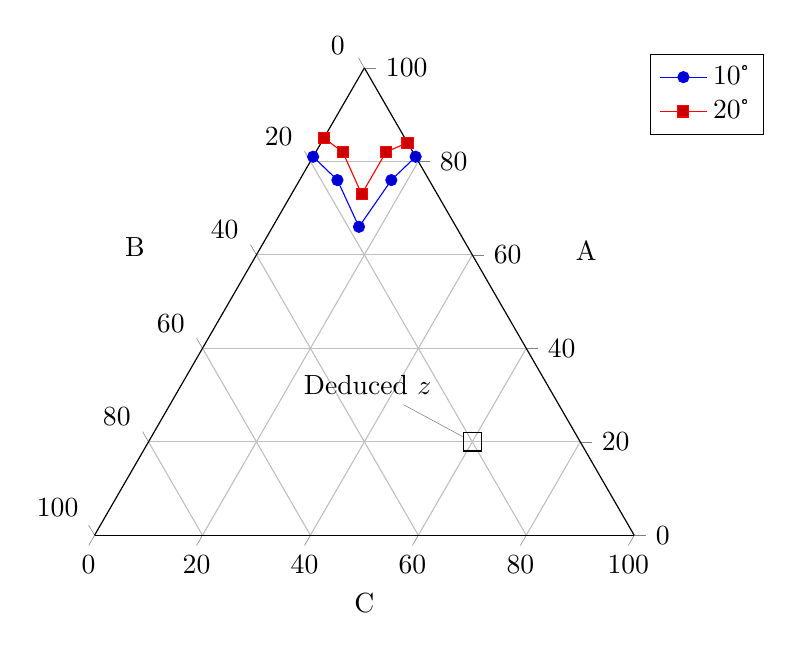
\begin{tikzpicture}
\begin{ternaryaxis}[xlabel=A,ylabel=B,zlabel=C]
	\addplot3 coordinates {
        (0.81,  0.19,  0.00)
        (0.76,  0.17,  0.07)
        (0.66,  0.16,  0.16)
        (0.76,  0.07,  0.17)
        (0.81,  0.00,  0.19)
	};

	\addplot3 coordinates {
        (0.85,  0.15,  0.00)
        (0.82,  0.13,  0.05)
        (0.73,  0.14,  0.13)
        (0.82,  0.06,  0.13)
        (0.84,  0.00,  0.16)
	};

	\node[pin=130:Deduced $z$,draw=black] at (axis cs:0.2,0.2) {};

	\legend{$10$\textdegree, $20$\textdegree}
\end{ternaryaxis}
\end{tikzpicture}
\end{document}
